% chapters/02_sections/gpu_architecture.tex
\section{GPU Architecture}\label{sec:gpu-architecture}

\subsection{Streaming Multiprocessor and Warp Execution}\label{sec:sm-warps}

The Streaming Multiprocessor (SM) is the fundamental compute unit of the GPU. Each 
A100 GPU contains 108 SMs, and all CUDA threads ultimately execute on one of them. 
Understanding the internal structure of an SM is essential for reasoning about 
occupancy, register pressure, and warp scheduling.

\begin{figure}[H]
  \centering
  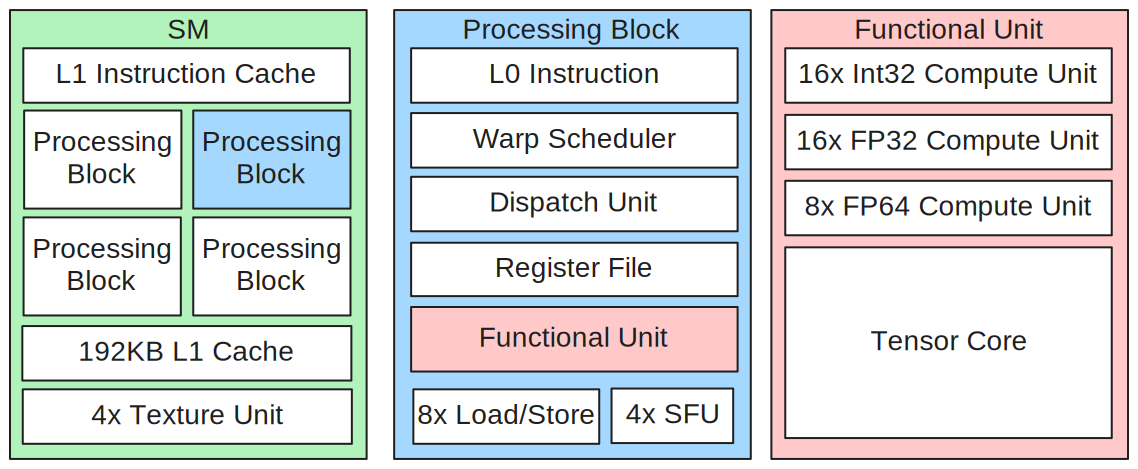
\includegraphics[width=0.95\textwidth]{SMBreakdown}
  \caption{Internal structure of an A100 Streaming Multiprocessor at three levels 
  of detail. \textbf{Left:} the SM contains four processing blocks sharing an L1 
  data cache and shared memory. \textbf{Centre:} each processing block includes a 
  warp scheduler, register file slice, execution units, LD/ST units, SFUs, and a 
  texture unit. \textbf{Right:} the execution units comprise 16 INT32 cores, 16 
  FP32 cores, 8 FP64 cores, and one tensor core.}
  \label{fig:sm-breakdown}
\end{figure}

Each SM is partitioned into four \emph{processing blocks} (also called 
sub-partitions). As shown in \cref{fig:sm-breakdown}, each processing block 
contains:

\begin{itemize}
  \item One \textbf{warp scheduler} with a single dispatch unit, capable of 
    issuing one instruction per cycle from the warp it selects.
  \item A slice of the \textbf{register file} (\num{16384} 32-bit registers 
    per block, \num{65536} per SM).
  \item \textbf{Execution units:} 16 INT32 cores, 16 FP32 cores, 8 FP64 
    cores, and one third-generation tensor core.
  \item \textbf{8 LD/ST units} for issuing memory load and store operations.
  \item \textbf{4 SFUs} (Special Function Units) for transcendental operations 
    such as \texttt{sin}, \texttt{exp}, and reciprocal square root.
  \item A \textbf{read-only/texture path} for cached read-mostly memory access.
  \item An \textbf{L0 instruction cache} private to the processing block.
\end{itemize}

The four processing blocks share the SM's L1 data cache and its configurable 
shared memory (up to \SI{164}{\kilo\byte} on the A100). Threads are grouped into 
\emph{warps} of 32 and assigned to processing blocks at launch time. Each warp 
scheduler selects one of its resident warps per cycle and issues a single 
instruction to the appropriate execution unit. Because the four schedulers operate 
independently, an SM can have four instructions from four different warps in flight 
simultaneously, which is the primary mechanism for hiding memory and instruction 
latency.

\subsection{Floating-Point Formats and Precision Trade-offs}\label{sec:fp-formats}

Scientific computing on GPUs has historically defaulted to 64-bit double precision (FP64), matching the convention established by decades of CPU-based numerical software. However, the A100 architecture supports a range of floating-point formats with dramatically different throughput characteristics, and for many workloads---including tensor contractions---FP32 or even reduced-precision formats offer sufficient accuracy at a fraction of the cost. This section reviews the relevant formats and motivates the precision choices made in this thesis.

\subsubsection{IEEE 754 Binary Representation}
The IEEE 754 standard~\cite{ieee754-2019} defines the binary floating-point formats used across virtually all modern hardware. Each format encodes a real number as
\begin{equation}\label{eq:ieee754}
  (-1)^{s} \times 2^{e - \text{bias}} \times (1 + f),
\end{equation}
where $s$ is a sign bit, $e$ is an unsigned integer stored in the exponent field, the \emph{bias} centres the exponent range around zero, and $f$ is the fractional part of the significand (with an implicit leading 1 for normal numbers). The three fields are packed into a fixed-width bit string as shown in \cref{tab:fp-bit-layout}. The bias can be computed as
\[
    2^{k - 1} - 1
\]
where $k$ is the number of exponent bits.

\begin{figure}[H]
  \centering
  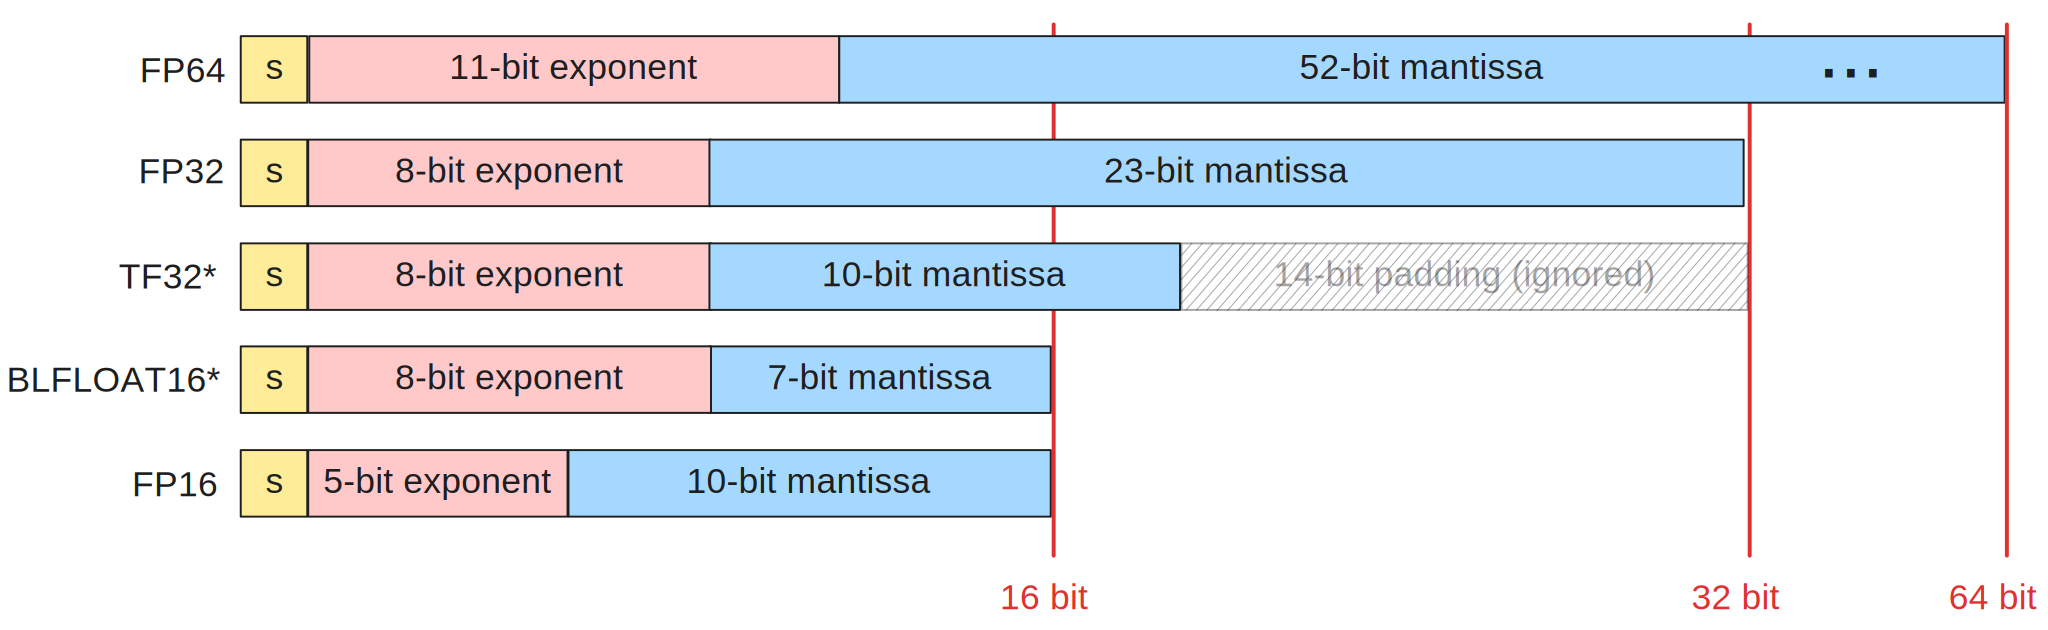
\includegraphics[width=0.9\textwidth]{FloatingPointBitComparions}
  \caption{Bit layout comparison of FP64, FP32, TF32, BF16, and FP16, with exponent and significand fields drawn to scale.}
  \label{fig:fp-bit-patterns}
\end{figure}

\begin{table}[H]
\centering
\caption{Bit layout of floating-point formats relevant to GPU computing. FP64, FP32, and FP16 are defined by IEEE 754~\cite{ieee754-2019}; BF16 and TF32 are industry-defined formats (see text). The mantissa column lists only the explicitly stored fraction bits; all formats carry an additional implicit leading bit for normal numbers.}
\label{tab:fp-bit-layout}
\begin{tabularx}{\textwidth}{l r r r r r}
\toprule
Format & Total bits & Sign & Exponent & Bias & Mantissa\footnotemark[1] \\
\midrule
FP64 (double) & 64 & 1 & 11 & 1023 & 52 \\
FP32 (single) & 32 & 1 & 8  & 127  & 23 \\
TF32           & 19 & 1 & 8  & 127  & 10 \\
BF16 (bfloat16)& 16 & 1 & 8  & 127  & 7  \\
FP16 (half)    & 16 & 1 & 5  & 15   & 10 \\
FP8 (E5M2)\footnotemark[2] & 8 & 1 & 5 & 15 & 2 \\
FP8 (E4M3)\footnotemark[2] & 8 & 1 & 4 & 7  & 3 \\
\bottomrule
\end{tabularx}
\footnotetext[1]{IEEE 754 uses the term \emph{significand}; \emph{mantissa} is used here as it is more widely recognised.}
\footnotetext[2]{FP8 formats are not supported on the A100 (Ampere); they were introduced with the H100 (Hopper) architecture.}
\end{table}

The number of exponent bits determines the \emph{dynamic range} (the ratio of the largest to smallest representable magnitudes), while the number of significand bits determines the \emph{precision} (the spacing between adjacent representable values). These properties are summarised in \cref{tab:fp-properties}.

\begin{table}[H]
\centering
\caption{Numerical properties of floating-point formats on the A100. Machine epsilon ($\varepsilon$) is the smallest increment to 1.0 that produces a distinct value, i.e.\ $\varepsilon = 2^{-p}$ where $p$ is the number of significand bits (including the implicit bit).}
\label{tab:fp-properties}
\begin{tabularx}{\textwidth}{l r r r}
\toprule
Format & Largest value & Smallest normal $>0$ & Machine epsilon \\
\midrule
FP64  & $\approx 1.8 \times 10^{308}$  & $\approx 2.2 \times 10^{-308}$ & $\approx 2.2 \times 10^{-16}$ \\
FP32  & $\approx 3.4 \times 10^{38}$   & $\approx 1.2 \times 10^{-38}$  & $\approx 1.2 \times 10^{-7}$  \\
TF32  & $\approx 3.4 \times 10^{38}$   & $\approx 1.2 \times 10^{-38}$  & $\approx 9.8 \times 10^{-4}$  \\
BF16  & $\approx 3.3 \times 10^{38}$   & $\approx 1.2 \times 10^{-38}$  & $\approx 7.8 \times 10^{-3}$  \\
FP16  & $65504$                         & $\approx 6.1 \times 10^{-5}$   & $\approx 9.8 \times 10^{-4}$  \\
\bottomrule
\end{tabularx}
\end{table}

Two aspects of this table merit attention. First, TF32 and BF16 share the same 8-bit exponent as FP32, so they retain the full FP32 dynamic range despite having far fewer significand bits. TF32 was introduced specifically for the Ampere tensor cores: inputs are stored as ordinary FP32 values, but the tensor core hardware internally truncates to 10 significand bits before performing the multiply-accumulate, with the accumulation itself carried out in full FP32~\cite{nvidia2020a100}. The programmer does not need to convert data explicitly; the truncation is transparent.

Second, FP16 has a severely limited dynamic range (maximum value $65504$), which makes it unsuitable for many scientific workloads without careful scaling. BF16 (``brain floating point''), originally developed for deep learning training on Google's TPUs~\cite{kalamkar2019bfloat16}, avoids this limitation by retaining the FP32 exponent range at the cost of reduced precision (7 fraction bits versus 10 for FP16).

\subsubsection{Examples}
\paragraph{Example: Encoding a decimal number in FP16.}
decimal number $0.15625_{10}$ has the binary representation $0.00101_2$ because
\[
  0.15625 = \frac{1}{8} + \frac{1}{32} = 0 \times 2^{-1} + 0 \times 2^{-2} + 1 \times 2^{-3} + 0 \times 2^{-4} + 1 \times 2^{-5}
\]
holds. To express this as an FP16 number we write it in normalised form,
\[
0.00101_2 = 1.01_2 \times 2^{-3},
\]
and match it against \cref{eq:ieee754}: the sign is $s = 0$ (positive), the true exponent is $-3$, and the stored exponent is $e = -3 + 15 = 12 = 01100_2$. The fraction field stores the bits after the implicit leading~1, i.e.\ $01$ padded with zeros to 10~bits. The complete bit representation is therefore
\[
  \underbrace{0}_{\text{sign}} \;|\; \underbrace{01100}_{\text{exp}} \;|\; \underbrace{0100000000}_{\text{mantissa}}.
\]

\paragraph{Example: Absorption in FP16 addition.}
Consider adding $1024.0$ and $0.5$ in half precision.
The value $1024.0 = 1.0 \times 2^{10}$ is stored as
\[
    \underbrace{0}_{\text{sign}} \;|\; \underbrace{11001}_{\text{exp}=25} \;|\; \underbrace{0000000000}_{\text{mantissa}},
\]
while $0.5 = 1.0 \times 2^{-1}$ is stored as
\[
    \underbrace{0}_{\text{sign}} \;|\; \underbrace{01110}_{\text{exp}=14} \;|\; \underbrace{0000000000}_{\text{mantissa}}.
\]
To perform the addition, the hardware aligns the exponents by shifting the smaller operand's significand to the right by $10 - (-1) = 11$ positions:
\[
    0.5 = \underbrace{0.00000000001}_{\text{11 places after the radix point}} \times 2^{10}.
\]
Since FP16 retains only 10 fraction bits after the implicit leading~1, the shifted significand falls entirely outside the representable precision and is rounded to zero. The result is $1024.0$---the smaller operand has been \emph{absorbed}.

Had the same computation been carried out in FP32 (23 fraction bits), the shift of 11~places is well within the available precision and the result is correctly obtained as $1024.5$. This example illustrates why mixed-precision strategies---performing arithmetic at higher precision than the storage format---can recover accuracy at modest cost.

\paragraph{Example: TF32 truncation in a matrix multiply.}
The A100 tensor cores accept FP32 inputs but internally truncate the significand from 23 to 10 fraction bits before performing the multiply, while the accumulation remains in full FP32. To see the effect, consider two $2 \times 2$ matrices with entries drawn from familiar constants:
\[
    A = \begin{pmatrix} 3.1415927 & 1.2345679 \\ 2.7182817 & 0.9876543 \end{pmatrix}, \qquad
    B = \begin{pmatrix} 0.9876543 & 2.7182817 \\ 1.2345679 & 3.1415927 \end{pmatrix}.
\]
After TF32 truncation, the entries lose their lower 13 significand bits:
\[
    \tilde{A} = \begin{pmatrix} 3.1406250 & 1.2343750 \\ 2.7167969 & 0.9873047 \end{pmatrix}, \qquad
    \tilde{B} = \begin{pmatrix} 0.9873047 & 2.7167969 \\ 1.2343750 & 3.1406250 \end{pmatrix}.
\]
The tensor core computes $C_{\text{TF32}} = \tilde{A}\,\tilde{B}$ with the multiplies at TF32 precision and the accumulation in FP32, giving
\[
    C_{\text{TF32}} =
    \begin{pmatrix} 4.6244 & 12.4091 \\ 3.9010 & 10.4817 \end{pmatrix},
\]
whereas exact FP32 arithmetic yields
\[
    C_{\text{FP32}} = A\,B =
    \begin{pmatrix} 4.6270 & 12.4182 \\ 3.9040 & 10.4919 \end{pmatrix}.
\]
The relative error in each entry is on the order of $5 \times 10^{-4}$ to $10^{-3}$, consistent with TF32's machine epsilon of $\varepsilon \approx 9.8 \times 10^{-4}$.

In practice, the entries of typical tensor contractions are not deliberately crafted to maximise the impact of truncation, and the FP32 accumulation across many products causes individual truncation errors to partially cancel. Empirical studies consistently report that TF32 is a drop-in replacement for FP32 in deep-learning training~\cite{nvidia2020a100}; whether the same holds for a given scientific workload must still be validated case by case in the benchmark chapter.

\paragraph{Remark: Fused multiply-add and single rounding.}
Modern GPU floating-point units implement the \emph{fused multiply-add} (FMA) operation
\[
    \operatorname{fma}(a, b, c) = \operatorname{round}(a \times b + c),
\]
where the product $a \times b$ is computed to \emph{full} (unrounded) precision before the addition and only a single rounding step is applied to the final result. By contrast, the non-fused sequence
\[
    t = \operatorname{round}(a \times b), \qquad r = \operatorname{round}(t + c)
\]
incurs two rounding errors. The difference is most visible when $a \times b$ and $c$ are of similar magnitude but opposite sign, so that their sum is much smaller than either operand.

As a concrete example, let $a = b = 1 + 2^{-12}$ and $c = -(1 + 2^{-11})$, all exactly representable in FP32. The exact product is
\[
    a \times b = (1 + 2^{-12})^2 = 1 + 2^{-11} + 2^{-24},
\]
so the exact result is $a \times b + c = 2^{-24} \approx 5.96 \times 10^{-8}$. In the non-fused path, the intermediate rounding of $a \times b$ to FP32 discards the $2^{-24}$ term (which is below one unit in the last place at magnitude ${\approx}\,1$), yielding $t = 1 + 2^{-11}$, and consequently $r = t + c = 0$---a complete loss of the true result. The FMA, retaining the full product before the addition, returns $2^{-24}$ correctly.

This property is directly relevant to tensor core computation: the multiply-accumulate $D = A \times B + C$ is implemented as a sequence of fused multiply-adds, and the single-rounding semantics mean that the accumulated dot products are more accurate than a na\"ive loop of separate multiplies and additions would be.

\subsubsection{A100 Throughput by Precision}\label{sec:a100-fp-throughput}

The performance gap between precisions is substantial. \Cref{tab:a100-throughput-by-format} reproduces the A100 throughput figures from NVIDIA's Ampere optimisation guide~\cite{nvidia2020gtc-ampere}, broken down by execution unit.

\begin{table}[H]
\centering
\caption{Peak floating-point throughput (TFLOPS) of the A100 by format and execution unit. Tensor core figures in parentheses include sparsity acceleration (2:4 structured sparsity). Data from~\cite{nvidia2020gtc-ampere}.}
\label{tab:a100-throughput-by-format}
\begin{tabularx}{\textwidth}{l r r r}
\toprule
Format & Scalar (CUDA cores) & Vector (CUDA cores) & Tensor cores \\
\midrule
FP64   & \num{9.7}  & \num{9.7}  & \num{19.5} \\
FP32   & \num{19.5} & \num{19.5} & \num{156} (TF32) \\
FP16   & \num{19.5} & \num{78}   & \num{312} (\num{624}) \\
BF16   & \num{19.5} & \num{39}   & \num{312} (\num{624}) \\
\bottomrule
\end{tabularx}
\end{table}

The ratios are stark. Moving from FP64 CUDA core arithmetic (\SI{9.7}{\tera\flops}) to FP32 (\SI{19.5}{\tera\flops}) doubles throughput at no algorithmic cost. Engaging the tensor cores in TF32 mode yields a further $8\times$ increase to \SI{156}{\tera\flops}, and FP16/BF16 tensor core throughput reaches \SI{312}{\tera\flops}---a $32\times$ factor over FP64. Even accounting for the fact that many kernels are memory-bandwidth-bound rather than compute-bound, the reduced data movement from using 32-bit instead of 64-bit values halves the memory traffic, which directly benefits bandwidth-limited operations.

\subsubsection{The Case for Single Precision in Tensor Network Computations}\label{sec:fp32-argument}

The choice of FP64 in scientific software is often driven by convention rather than necessity~\cite{higham2022mixed}. Double precision provides roughly 15--16 decimal digits of accuracy, while single precision provides 7--8. Whether the additional digits matter depends on the conditioning of the computation and the accuracy actually required by the application. Higham and Mary~\cite{higham2022mixed} survey a broad class of numerical linear algebra algorithms where mixed- or reduced-precision arithmetic achieves results of comparable quality to FP64 at substantially lower cost---an observation that applies directly to the tensor contractions considered here.

For tensor network algorithms, several factors favour FP32:

\begin{enumerate}
  \item \textbf{Physical observables are approximate.} Tensor network methods are inherently approximate---the bond dimension truncation introduces controlled errors that typically far exceed single-precision rounding. When the truncation error is $\BigO(10^{-4})$ to $\BigO(10^{-6})$, carrying $10^{-16}$ precision in every floating-point operation is wasteful.
  \item \textbf{Iterative refinement.} Many tensor network algorithms are iterative (e.g.\ DMRG sweeps, variational optimisation). Rounding errors from FP32 arithmetic are corrected at each iteration, so they do not accumulate in the same way as in a single long computation.
  \item \textbf{Memory pressure.} Tensors with large bond dimensions consume substantial memory. Halving the per-element storage from 8 bytes to 4 bytes doubles the tensor sizes that fit in GPU memory, or equivalently allows larger bond dimensions for the same memory budget.
  \item \textbf{Bandwidth amplification.} Since tensor contractions are frequently memory-bandwidth-bound (\cref{sec:gpu-memory-hierarchy}), the $2\times$ reduction in data movement from FP32 translates almost directly into a $2\times$ speedup for bandwidth-limited kernels, before accounting for any compute throughput gains.
\end{enumerate}

The combination of these factors yields a practical speedup well in excess of the raw $2\times$ compute ratio, as demonstrated in the benchmarks in \cref{ch:results}. Where necessary, mixed-precision strategies---accumulating in FP32 while storing in FP16 or BF16---can push performance further (see~\cite{higham2022mixed} for a rigorous treatment), though this thesis focuses on FP32 as the primary working precision.

\subsection{Memory Hierarchy}\label{sec:gpu-memory-hierarchy}
\begin{figure}[H]
  \centering
  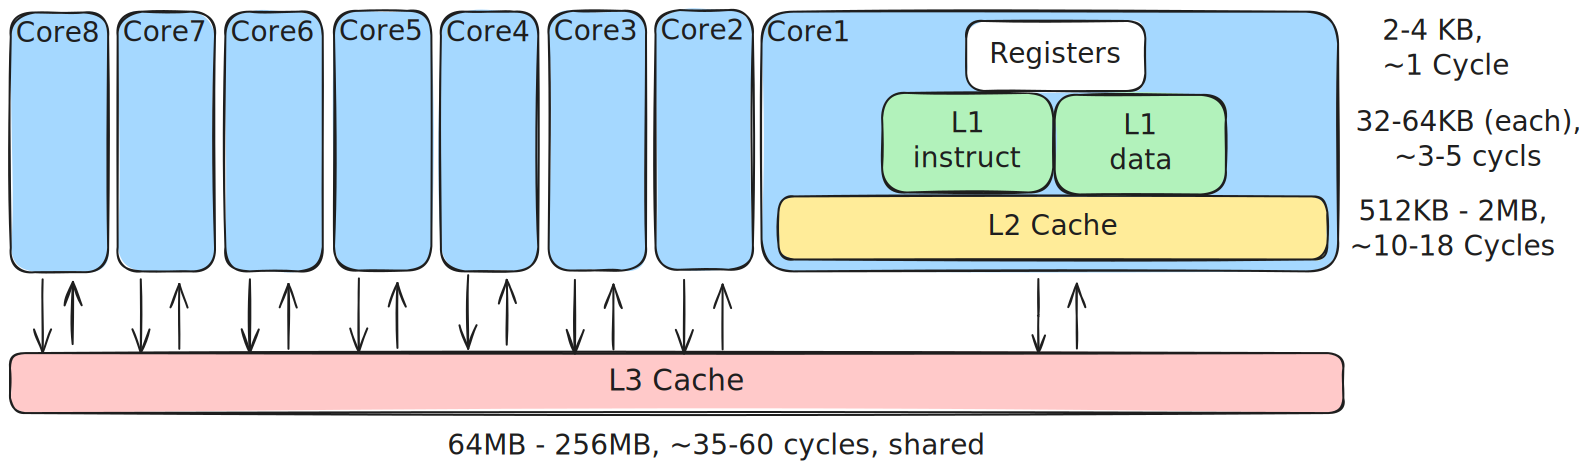
\includegraphics[width=0.9\textwidth]{CPUCacheHierarchy}
  \caption{Memory hierarchy of a modern CPU, showing the register file and cache levels (L1, L2, L3) before main memory (DRAM).}
  \label{fig:cpu-cache-hierarchy}
\end{figure}
As shown in \cref{fig:cpu-cache-hierarchy}, modern CPUs rely on a deep cache hierarchy to reduce effective memory latency.


\paragraph{GPU Memory Hierarchy}
\begin{figure}[H]
  \centering
  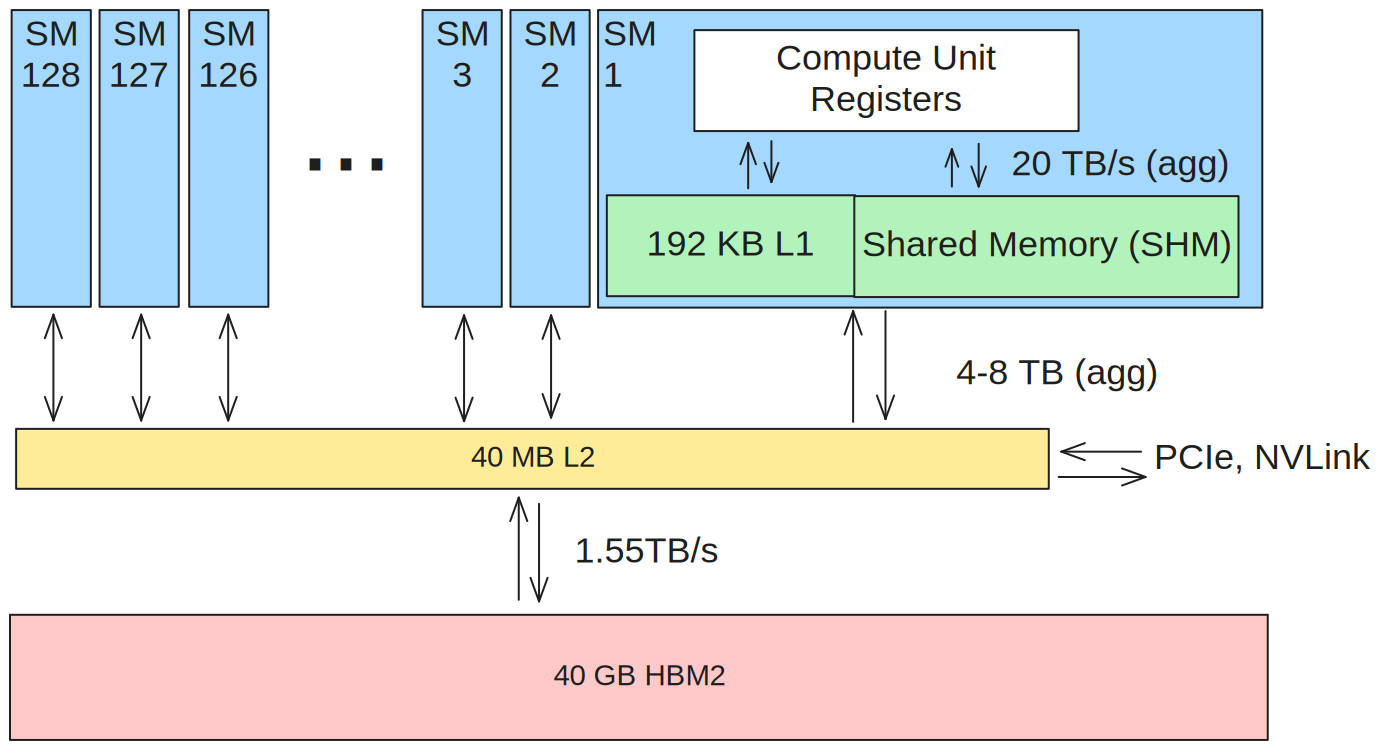
\includegraphics[width=0.65\textwidth]{A100CacheHierarchy}
  \caption{Memory hierarchy of an A100 GPU, showing registers, shared memory/L1, L2 cache, and HBM global memory.}
  \label{fig:a100-cache-hierarchy}
\end{figure}

Where CPUs use deep cache hierarchies to hide latency, GPUs prioritise bandwidth and expose a shallower hierarchy tuned for throughput. Four levels are relevant:

\begin{itemize}
  \item \textbf{Registers} reside in the SM and offer single-cycle access. They are private to each thread and are the scarcest on-chip resource: the number of registers a kernel uses directly limits occupancy.
  \item \textbf{Shared memory} is also on-chip but visible to all threads in a block, making it the primary mechanism for explicit data reuse and inter-thread communication. Most high-performance kernels---tiled matrix multiplications, tensor contractions---stage data through shared memory to avoid repeated global loads.
  \item \textbf{L2 cache} is shared across all SMs and transparently caches global memory traffic. On the A100 it is \SI{40}{\mega\byte}, modest relative to the core count, which reflects the throughput-oriented design.
  \item \textbf{HBM (global memory)} provides the bulk storage. The A100-SXM4-40GB used in this thesis provides \SI{40}{\giga\byte} HBM with a peak bandwidth of approximately \SI{1555}{\giga\byte\per\second} (\cref{tab:a100-specs}). Access latency, however, is roughly $500\times$ that of a register access (\cref{tab:a100-memory-latency}).
\end{itemize}

The practical consequence is that most scientific GPU kernels, including tensor contractions, are memory-bandwidth-bound rather than compute-bound. Performance therefore hinges on maximising reuse in registers and shared memory and accessing HBM in coalesced, bandwidth-efficient patterns.

\subsection{NVIDIA A100 Ampere Architecture}\label{sec:a100}
\subsubsection{Hardware Overview}

\begin{table}[H]
\centering
\caption{Key hardware specifications of the NVIDIA A100 (SXM4-40GB baseline).}
\label{tab:a100-specs}
\begin{tabularx}{\textwidth}{X r}
\toprule
Property & Value \\
\midrule
Streaming Multiprocessors (SMs) & \num{108} \\
CUDA cores per SM & \num{64} \\
Tensor cores per SM & \num{4} \\
Warp schedulers per SM & \num{4} \\
Maximum threads per SM & \num{2048} \\
Maximum warps per SM & \num{64} \\
Maximum blocks per SM & \num{32} \\
Register file size per SM (32-bit registers) & \num{65536} \\
Shared memory per SM (KB) & \num{164} \\
L2 cache size (MB) & \num{40} \\
HBM memory capacity (GB) & \num{40} \\
Peak memory bandwidth (GB/s) & \num{1555} \\
Base clock frequency (GHz) & \num{1.41} \\
\bottomrule
\end{tabularx}
\end{table}

The A100 employs high-bandwidth memory as its main device memory, providing the throughput required to sustain dense linear algebra kernels.

\subsubsection{Theoretical Peak Performance}

\begin{table}[H]
\centering
\caption{Theoretical peak floating-point throughput of the A100 GPU.}
\label{tab:a100-peak-performance}
\begin{tabularx}{\textwidth}{X r r}
\toprule
Precision & Peak TFLOPS & Relative speed \\
\midrule
FP64 (CUDA cores) & \num{9.7} & 1.0$\times$ \\
FP64 (Tensor cores) & \num{19.5} & 2.0$\times$ \\
FP32 & \num{19.5} & 2.0$\times$ \\
TF32 (Tensor cores) & \num{156.0} & 16.1$\times$ \\
FP16 (Tensor cores) & \num{312.0} & 32.2$\times$ \\
\bottomrule
\end{tabularx}
\end{table}


\subsubsection{Derived Performance Limits}

\begin{table}[H]
\centering
\caption{Derived theoretical limits of the A100 architecture.}
\label{tab:a100-derived}
\begin{tabularx}{\textwidth}{X r}
\toprule
Metric & Value \\
\midrule
Peak FP32 performance per SM (TFLOPS) & \num{0.18} \\
Peak FP64 performance per SM (TFLOPS) & \num{0.09} \\
Tensor core FP16 performance per SM (TFLOPS) & \num{2.89} \\
Memory bandwidth per SM (GB/s) & \num{14.40} \\
Total CUDA cores & \num{6912} \\
Total FP64 cores & \num{3456} \\
Maximum resident warps & \num{6912} \\
Maximum resident threads & \num{221184} \\
Arithmetic intensity threshold FP32 (FLOPs/byte) & \num{12.5} \\
Arithmetic intensity threshold FP64 (FLOPs/byte) & \num{6.2} \\
\bottomrule
\end{tabularx}
\end{table}


\subsubsection{Memory Latency}

\begin{table}[H]
\centering
\caption{Approximate memory access latency at different hierarchy levels.}
\label{tab:a100-memory-latency}
\begin{tabularx}{\textwidth}{X r}
\toprule
Memory level & Latency (cycles) \\
\midrule
Registers & \num{1} \\
Shared memory & \num{20} \\
L2 cache & \num{200} \\
HBM global memory & \num{500} \\
\bottomrule
\end{tabularx}
\end{table}

\subsection{Compute Node Topology}\label{sec:node-topology}

The performance of GPU-accelerated applications depends not only on the GPU itself but also on the topology of the compute node---how CPUs, GPUs, and memory are interconnected. This subsection describes the node architecture of the JURECA-DC system used throughout this thesis, which is representative of modern multi-GPU HPC nodes.

\subsubsection{CPU and NUMA Topology}

Each compute node contains two AMD EPYC 7742 processors (Rome, Zen\,2
microarchitecture), each with 64 physical cores. The chips follow a chiplet
design. Since the terms are easy to mix up, we fix the naming used in this
thesis:

\begin{itemize}
  \item \textbf{CCD} (\emph{Core Complex Die}): a compute chiplet containing CPU cores.
  \item \textbf{CCX} (\emph{Core Complex}): a core cluster inside a CCD. On
    EPYC\,7742, each CCD has two CCXes.
  \item \textbf{cIOD} (\emph{central I/O die}): the central die that provides
    memory controllers, PCIe root complexes, and fabric routing.
\end{itemize}

On this Rome generation, each CCX contains four cores with a private
\SI{16}{\mega\byte} L3 cache. The hierarchy is shown in
\cref{fig:numa-cpu-node}.

\begin{figure}[H]
  \centering
  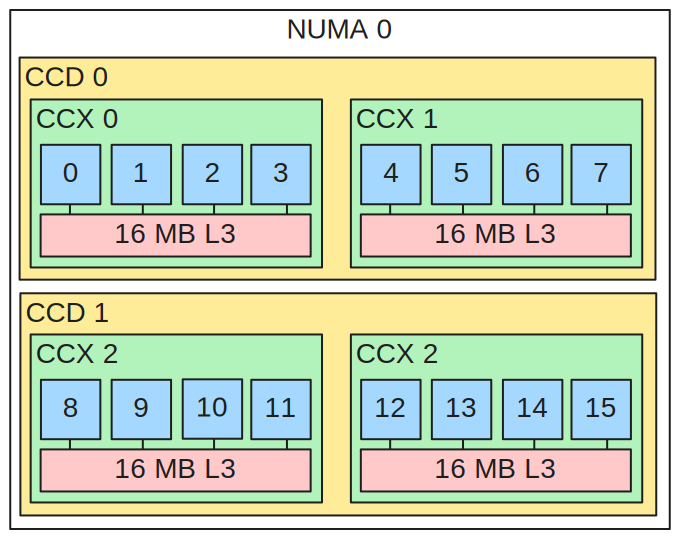
\includegraphics[width=0.5\textwidth]{NumaCPUNode}
  \caption{NUMA and chiplet hierarchy of a single AMD EPYC 7742 socket. Each socket contains 8 CCDs grouped into 4 NUMA domains (NPS=4 configuration). Each CCD holds two CCXes, each with 4 cores and a private \SI{16}{\mega\byte} L3 cache. All CCDs connect to a central I/O die that houses the memory controllers and PCIe root complexes.}
  \label{fig:numa-cpu-node}
\end{figure}

The BIOS is configured with NPS=4, which exposes four NUMA domains per socket
(eight in total across the node). Each NUMA domain encompasses two CCDs (16
cores, 32 threads with SMT) and a quarter of the socket's memory controllers.
This configuration allows the operating system and runtime to make NUMA-aware
allocation decisions.

\paragraph{Infinity Fabric and latency classes.}
AMD's Infinity Fabric connects CCX/CCD resources to the cIOD and also connects
the two sockets. The practical latency hierarchy for software placement
decisions is:

\begin{enumerate}
  \item \textbf{Intra-CCX:} cores sharing the same \SI{16}{\mega\byte} L3 cache communicate through it at low latency.
  \item \textbf{Cross-CCX / cross-CCD, same socket:} communication no longer
    benefits from a shared L3 and is routed via Infinity Fabric through cIOD
    resources, with higher latency.
  \item \textbf{Cross-socket:} traffic traverses inter-socket Infinity Fabric
    links (xGMI), which is the highest-latency path.
\end{enumerate}

\paragraph{Why this matters for GPU work.}
The GPU is not attached directly to a random core; it is attached to a PCIe
root complex on the cIOD, and each GPU therefore has a \emph{local} NUMA region
on the host side. A host-to-device transfer is fastest when both the launching
thread and the source host memory are local to the GPU-affine NUMA domain.

If either thread placement or host-memory placement is remote, the transfer must
take additional Infinity Fabric hops before reaching PCIe, which increases
latency and can reduce effective bandwidth.

\subsubsection{GPU Interconnect Topology}

Each node has four NVIDIA A100-SXM4-40GB GPUs arranged in a fully connected mesh via NVLink\,3.0. Every GPU pair is connected by four NVLink bridges (denoted NV4 in NVIDIA's topology notation), providing \SI{100}{\giga\byte\per\second} of uni-directional bandwidth between any two devices. This symmetric, all-to-all connectivity means that multi-GPU tensor contractions do not suffer from topology-dependent bandwidth asymmetries.

Each GPU is physically attached via PCIe Gen\,4 $\times$16 to a specific NUMA domain on one of the two CPU sockets:

\begin{table}[H]
\centering
\caption{GPU-to-NUMA affinity on a JURECA-DC compute node.}
\label{tab:gpu-numa-affinity}
\begin{tabular}{l l l l}
\toprule
GPU & Socket & NUMA domain & CPU cores (physical) \\
\midrule
GPU\,0 & 0 & 3 & 48--63 \\
GPU\,1 & 0 & 1 & 16--31 \\
GPU\,2 & 1 & 7 & 112--127 \\
GPU\,3 & 1 & 5 & 80--95 \\
\bottomrule
\end{tabular}
\end{table}

The full topology, including the three classes of CPU--GPU data paths, is illustrated in \cref{fig:gpu-topology}. 

\begin{figure}[H]
  \centering
  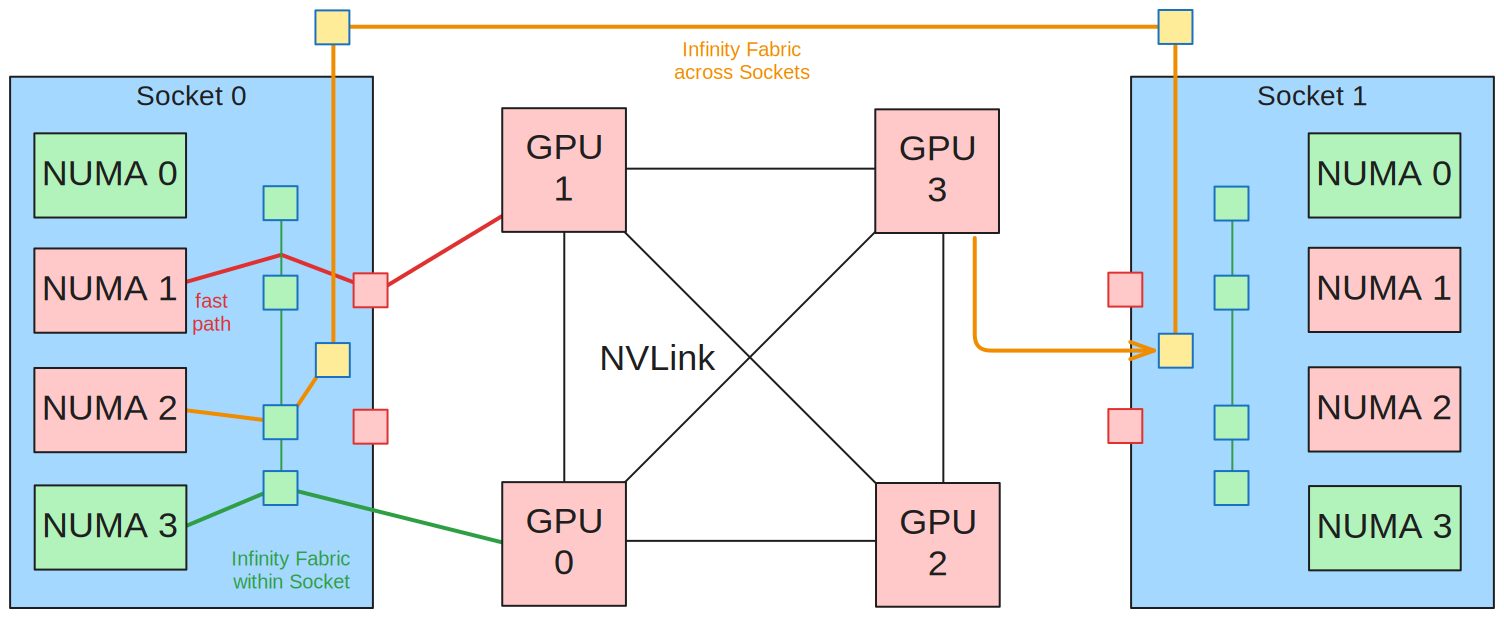
\includegraphics[width=0.9\textwidth]{GPUTopology}
  \caption{Compute node topology showing the four A100 GPUs (centre) connected via NVLink\,3.0, with the two CPU sockets on either side. Three representative host--device paths are highlighted: a fast local PCIe path (GPU\,1 $\leftrightarrow$ NUMA\,1), an intra-socket Infinity Fabric path (GPU\,0 $\leftrightarrow$ NUMA\,3), and a cross-socket Infinity Fabric path (GPU\,3 $\leftrightarrow$ NUMA\,2).}
  \label{fig:gpu-topology}
\end{figure}

The distinction between these paths matters for host--device data transfers. A \texttt{cudaMemcpy} initiated from a CPU thread pinned to a GPU's local NUMA domain takes the shortest PCIe path through the I/O die. If the source thread or memory allocation resides on the wrong NUMA domain---or worse, the wrong socket---the transfer must additionally traverse Infinity Fabric, increasing latency. For GPU-to-GPU communication, NVLink bypasses the CPU subsystem entirely, making the CPU topology irrelevant for peer-to-peer transfers.

\paragraph{Fast-path policy used in this thesis.}
For runs that include host-device staging, the following policy is applied:
\begin{enumerate}
  \item pin the orchestration thread to cores in the GPU-affine NUMA domain,
  \item allocate pinned host buffers on the same NUMA domain,
  \item execute \texttt{cudaMemcpyAsync} from that thread/context to preserve
    the local PCIe path.
\end{enumerate}

This is a standard NUMA-locality rule for PCIe-attached accelerators and is
independent of tensor-network physics details.
More tightly integrated CPU--GPU systems (e.g.\ Grace-Hopper style designs) use
different host-device topology assumptions and are therefore outside the scope
of this node-level model.

\paragraph{Host-device path cost model.}
For a transfer of size $V$ bytes, a useful first-order model is
\[
  T_{\mathrm{H2D}}(\pi, V)
  \approx
  T_0(\pi) + \frac{V}{B_{\mathrm{eff}}(\pi)},
\]
where $\pi$ is the path class (local, same-socket remote, or cross-socket
remote), $T_0$ is the fixed setup/latency term, and $B_{\mathrm{eff}}$ is the
effective end-to-end bandwidth.

To make the topology penalty explicit, we can write
\[
  T_0(\pi) = T_0^{\mathrm{local}} + n_{\mathrm{IF}}(\pi)\,\tau_{\mathrm{IF}},
\]
with $n_{\mathrm{IF}}$ the number of additional Infinity Fabric segments and
$\tau_{\mathrm{IF}}$ an average per-segment latency penalty. In practice, this
gives the expected ordering
\[
  T_{\mathrm{local}} < T_{\mathrm{same\ socket\ remote}} < T_{\mathrm{cross\ socket}}.
\]
This model is intentionally simple, but it is sufficient for placement policy
decisions: thread pinning and host-buffer NUMA placement should minimise
$n_{\mathrm{IF}}$ and maximise $B_{\mathrm{eff}}$.

In practice, this topology has two implications for the work in this thesis:

\begin{itemize}
  \item \textbf{Single-GPU kernels:} the CPU topology is largely invisible, since kernel launch overhead is small and tensor data resides in GPU memory throughout the computation.
  \item \textbf{Multi-GPU contractions:} data distribution and inter-GPU communication use NVLink exclusively. Host-side orchestration threads are pinned to the appropriate NUMA domain to minimise any residual host--device transfer overhead.
\end{itemize}
